\documentclass[a4paper, 12pt]{article}
% use UTF8 encoding
\usepackage[utf8]{inputenc}
% use KoTeX package for Korean
\usepackage{kotex}
% for multiple columns
\usepackage{multicol}

% for poem typing
\usepackage{verse}
% for multiple columns
\usepackage{multicol}

% for poem typing
\usepackage{verse}

\usepackage{tikz}
\usetikzlibrary{automata, arrows, calc, positioning}

\title{Multilayered Classifier}
\author{Wye}

\begin{document}
    \maketitle
    \newpage

    \section*{Understanding Frame}
    \paragraph*{This is not good.} 
    I had some problem regarding understanding machine learning precess
    mainly due to unclear internal computing steps hidden in the frame. 
    It seems to me that altering and improving frame was nearly impossible
    to do, and besides,
    its obscure operating seems likely to be vaporized so easily in my head
    that it was hard for me to grasp its essence.

    \paragraph*{It's time to understanging fuzzy frame in hard way.}
    It's more like I rebuild the frame from the beginning. Of course,
    with the help of some texts and advices.\cite{saito2017deep}

    \section{Main Data(Feature Records) Shapes}
    \paragraph{How should data flow in the process?}
    This is about main theory of perceptron machine learning process. It can be 
    dissected to some stages. 
    \subsection*{Nodes States} 
    How do we set $X$, $W_k$ values and produce $Y_k$, $Z$? 
    Layer of a perceptron is a node of tuple $(W_k, h\circ  \Sigma)$, 
    where $W_k$ is a weight matrix, $h$ activate function, $\Sigma$ 
    weigted sum, and $h\circ  \Sigma$ mean composite of the two. Fianlly,
    $X$, $Y_k$ are input and outputs respectively.
    \subsubsection{So we need classify the multi-layered neural network of that states,}
    i.e. \emph{State} class MultiLayeredNet


    \subsection*{Learning Dynamics}

    \begin{figure}
        \centering
        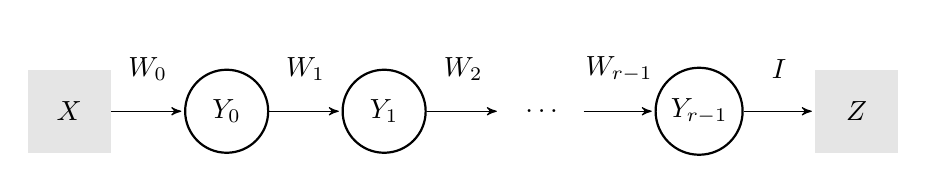
\begin{tikzpicture} [->, >=stealth',shorten >=1pt,auto,
            node distance=2.5cm,scale=1, transform shape,
            align=center,minimum size=3em]
            

            \tikzstyle{data} = [rectangle, fill=black!10]
            \tikzstyle{layer} = [circle, draw=black, thick]
            \tikzstyle{ellipsis} = []

            \node[data](input) at(0, 0) {$X$};
            \node[layer](layer_0) at(2, 0) {$Y_0$};
            \node[layer](layer_1) at(4, 0) {$Y_1$};
            \node[ellipsis](ellipsis) at(6, 0) {$\ldots$};
            \node[layer](layer_r-1) at(8, 0) {$Y_{r-1}$};
            \node[data](output) at(10, 0) {$Z$};

            \path (input) edge node {$W_0$} (layer_0)
                (layer_0) edge node {$W_1$} (layer_1)
                (layer_1) edge node {$W_2$} (ellipsis)
                (ellipsis)edge node {$W_{r-1}$} (layer_r-1)
                (layer_r-1) edge node {$I$}(output)
            ;
       \end{tikzpicture} 
       \caption{\emph{Multi-layered neural network:}
                The overall structure of a $r$-layered Neural Network looks like this.
        }
    \end{figure}
    
    \vspace{20pt}
    \begin{table}
        \centering
        \begin{tabular}{| l c c c c c c c |}
            \hline
             & $X$       & $W_0$     & $Y_0$   & $\ldots$ & $W_{r-1}$  & $Y_{r-1}$ & $Z$ \\
            \hline
            shape    & $(m, n)$ & $(n, k_0)$ & $(m, k_0)$ & $\ldots$ & $(k_{r-2}, \ell)$ & $(m, \ell)$ & $(m,\ell)$ \\%& $\(n, k_0\)$ & $\(k_{r-2}, l\)$ & $\(l,\)$ \\
            \hline
        \end{tabular}
        \caption[a]{shapes}
    \end{table}

    \bibliographystyle{abbrv}
    \bibliography{../../ref_bib/light.bib}
\end{document}